% *********************************************************************
% © 2021–2024 Jeremy Sylvestre
%
% Permission is granted to copy, distribute and/or modify this document
% under the terms of the GNU Free Documentation License, Version 1.3 or
% any later version published by the Free Software Foundation; with no
% Invariant Sections, no Front-Cover Texts, and no Back-Cover Texts. A
% copy of the license is included in the appendix entitled “GNU Free
% Documentation License” that appears in the output document of this
% PreTeXt source code. All trademarks™ are the registered® marks of
% their respective owners.
%
% *********************************************************************

\newcommand*{\xmin}{-2}
\newcommand*{\xmax}{2}
\newcommand*{\ymin}{-4}
\newcommand*{\ymax}{12}

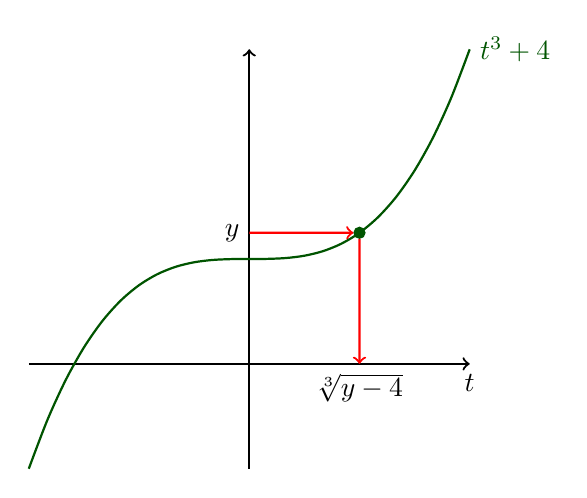
\begin{tikzpicture}
[
	closedpt/.style={circle,draw,fill,inner sep=0pt,minimum size=4pt},
	openpt/.style={circle,draw,inner sep=0pt,minimum size=4pt},
	yscale=0.333,xscale=1.4
]

	% axes
	\draw[->,thick] (\xmin,0) -- (\xmax,0) node[below] {$t$};
	\draw[->,thick] (0,\ymin) -- (0,\ymax);

	\draw[green!33!black,thick,domain=-2:2,smooth] plot (\x,{\x * \x * \x + 4}) node[right] {$t^3 + 4$};

	\node[closedpt,green!33!black] at (1,5) (pt) {};

	\draw[red,thick,->] (0,5) -- (pt);
	\draw[red,thick,->] (pt) -- (1,0);


	\node[below] at (1,0) {$\sqrt[3]{y - 4}$};
	\node[left] at (0,5) {$y$};

\end{tikzpicture}
